\section{Asynchronous Subsystems}
The nature of Order's requires a vary particular type of asynchronous handling.  Lucky for us we were able to find a ruby gem that makes this messy process quite elegant.  Resque allows one to queue up tasks and execute them in "first in first out"(FIFO) order by dequeueing the next enabled task in-line and performing it.  For our application we need to be able to wait before processing certain orders based on their dependencies and characteristics.  Rather then have a different data-type and handler for every type of order, we took the approach to consolidate all order types into a single order data-type that has a field that specifies the transactionType.  The orderHandler can be considered more of a wrapper function as it checks the transactionType of the order it is to perform and send it off to be handled uniquely based on the checked value.  While market orders, are executed almost immediately after being placed, stop and limit orders may not be executed for quite some time.  Whenever a task needs to be performed asynchronously, the task is entered into a designated portion of a Redis database, configured as a queue. Background "workers" (processes) perform tasks as they arrive. Tasks can also be scheduled to occur at specific times or intervals. In this way, everything from polling the data-stream for stock updates to performing scheduled updates and e-mails can be coordinated by a single system.


\subsection{Asynchronous Subsystem Diagram}
\begin{figure}[H]
\centering
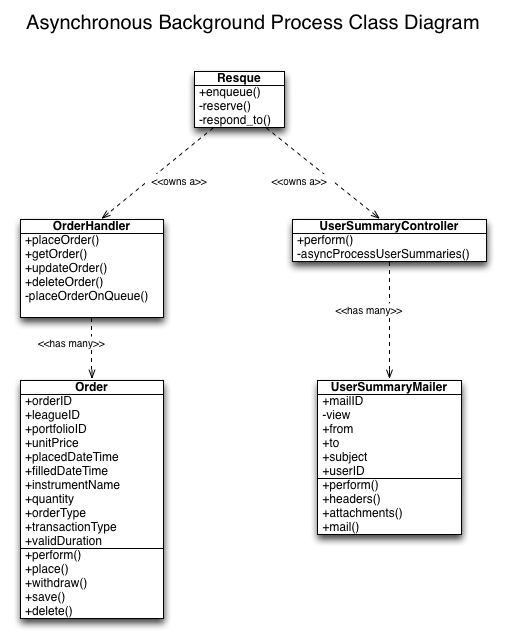
\includegraphics[width=5in]{./Diagrams/ClassDiagrams/cd.png}
\caption{ Asynchronous Class Diagrams.}
\end{figure}

\subsection{Attribute Table}
\begin{table}
\begin{tabular}{|p{3in}|p{3in}|p{3in}|}
\hline
Concept & Attribute & Meaning\\
\hline
Task Queue & resque & resque is a ruby gem that queue's Order Handling jobs and processes them first in first out.\\
\hline
Order Handler & orderHandler & function responsible for processing orders.\\
\hline
Order & order & data type that contains order details to be processed by the orderHandler.\\
\hline
Mail Controller & UserSummaryController & handles queueing userSummaryMailer tasks and then executing them.\\
\hline
Mail Sender & UserSummaryMailer & handles the generation and sending of a single User Summary.\\
\hline
\end{tabular}
\caption{ Attribute Table.}
\end{table}
